
\begin{frame}{Setup for the explosion}	

We tried several parameters
\begin{itemize}
\item Size of the explosion centre
\item Pressure difference 
\item Location of the explosion
\end{itemize}
\vspace{1cm}
        	  	\begin{minipage}{0.3\textwidth}
        	  	\begin{block}{}
        	  				\vspace{-1.7cm}
        	  	     	  	\begin{figure}
        	  	     	  	      	  \centering
        	  	     	  	      	  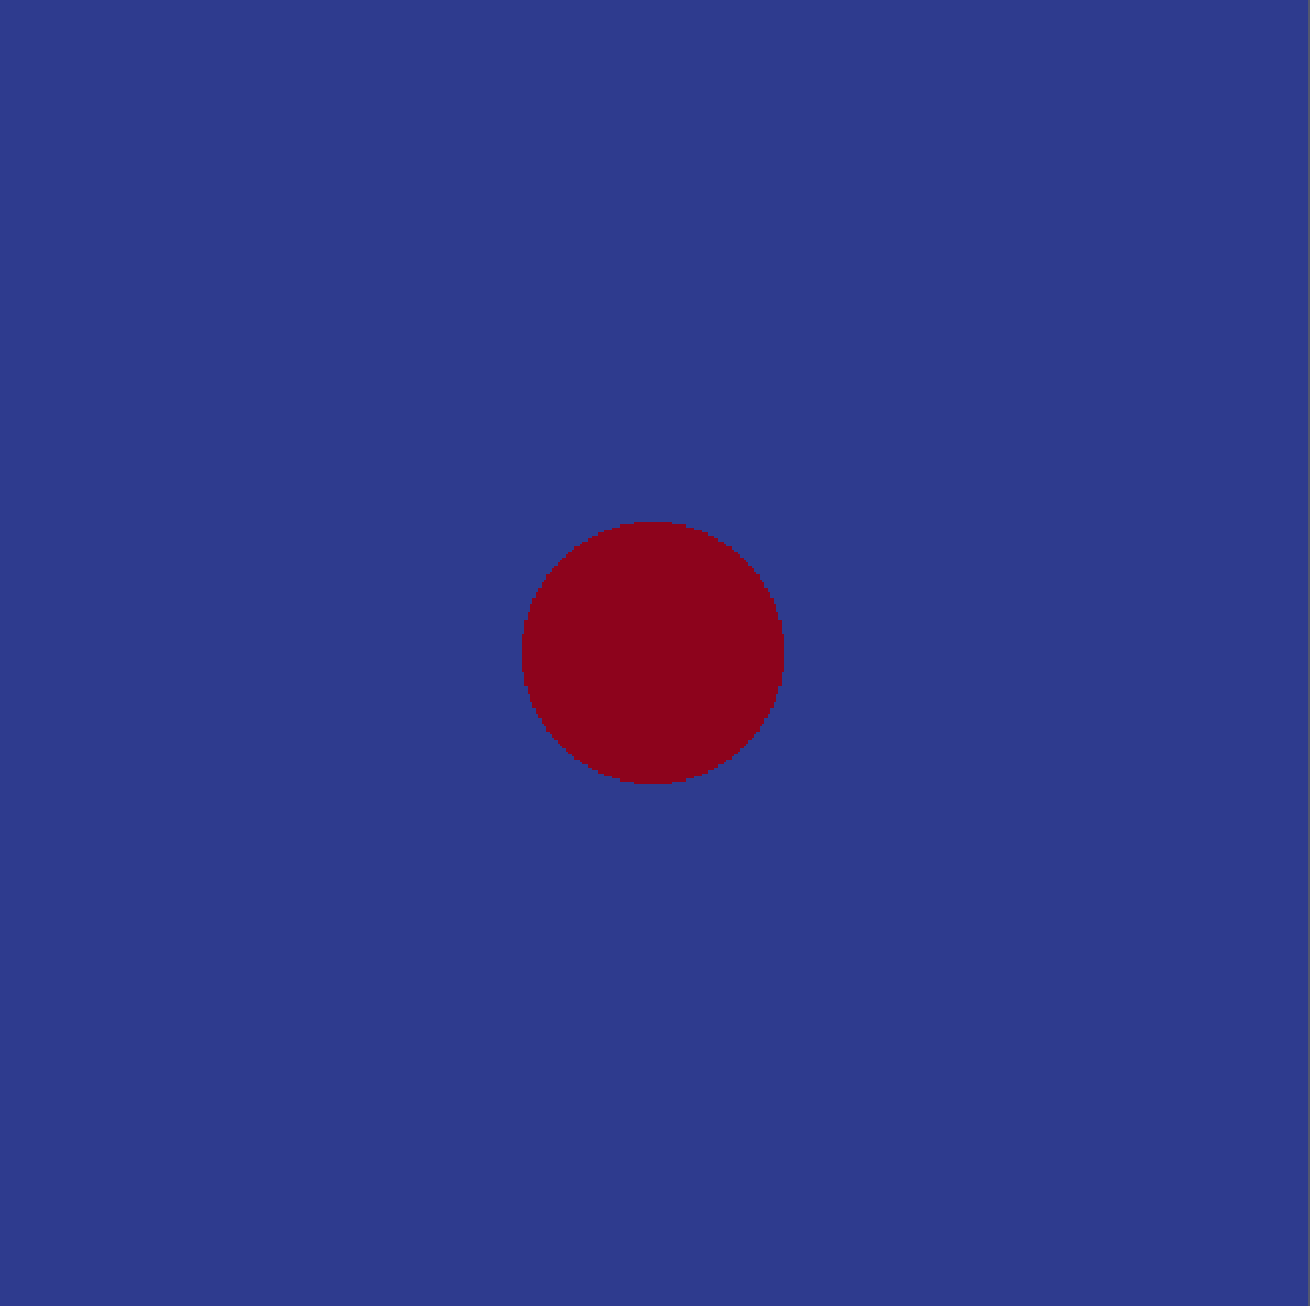
\includegraphics[width=\textwidth]{../../figs/exp/circ}
        	  	     	  	 \end{figure}
        	  	\end{block}
        	  	\end{minipage}
        	  	\begin{minipage}{0.3\textwidth}
        	  			\begin{block}{}
        	  			\vspace{-1.7cm}
        	  				\begin{figure}
        	  						\centering
        	  						
\includegraphics[width=\textwidth]{../../figs/exp/sqr}
        	  					\end{figure}
        	  		  	\end{block}
        	  	\end{minipage}
				\begin{minipage}{0.3\textwidth}
        	  			\begin{block}{}
        	  			\vspace{-1.7cm}
        	  				\begin{figure}
        	  						\centering
        	  						
\includegraphics[width=\textwidth]{../../figs/exp/corner}
        	  					\end{figure}
        	  		  	\end{block}
        	  	\end{minipage}
\end{frame}

\begin{frame}{Comparing two explosions}

Play the movie

\end{frame}

\begin{frame}{3d rayleigh taylor}



\end{frame}








	